\chapter{システムの概要}
\label{chp:third}
本章では，私の提案する手法について説明する．
本研究では，2枚の画像から分割した画像（駒）を元に新たに「合成駒」生成し，それを用いてスライディングブロックパズルを作る．
この駒を用いたパズルを，決められた配置になるように解くことによって，一方の画像からもう一方の画像に変化するアニメーションを表示させるものである．
まずは，システム全体の流れを簡単に説明する．
\begin{enumerate}
    \item パズルを解く前（以下original画像）と後（以下target画像）の近似させる2枚の画像を入力とする．
    \item original画像，target画像それぞれをグレースケール変換し，それぞれを$n \times n$個の画像（駒）に分割する．
    \item original画像の駒とtarget画像の駒とで合成駒を生成するための組み合わせ（配置）を決める．
    \item 組み合わせから，$n \times n$個の合成駒を生成し，original画像に割り当てる．
    \item 配置からのスライディングブロックパズルを解くアニメーションを出力する．
\end{enumerate}
以下で，画像処理，パズル表示の二つに分けて詳しく説明する．
\section{画像処理}
\label{sec:imgsolve}
ここでは，上記の1〜3の手順について説明する．
本論文では，画像は全てbitmap形式で扱う．前提知識として以下に説明する．\\
\textbf{bitmap画像}

    bitmap画像（図\ref{fig:gena}参照）とは，コンピュータグラフィックスにおける画像の形式のひとつであり，
    画像をピクセルと呼ばれる格子状の細密な点に分割し，その点の色や濃度を$RGB$等の表色系を用いて数値として表現しているものである．
    bitmapのbitというのはこれらの数値をbitで管理しているからである．
    わかりやすい例がドット絵であり，言い換えるならば，ピクセルが判別できるほど解像度の低いbitmap画像である．
    以下では，R(赤)値を$r$,G(緑)値を$g$,B(青)値を$b$とする．一般的な24bit bitmapでは，各ピクセルが0〜255（256段階）の$r$,$g$,$b$の数値を持ち，
    赤256段階$\times$緑256段階$\times$青256段階＝16,777,216色を表現することができる．
    \begin{figure}[H]
        \centering
        \includegraphics[width=10cm]{./fig/Gena.png}
        \caption{bitmap画像}
        \label{fig:gena}
    \end{figure}
    \noindent
    \textbf{1．original画像とtarget画像の二枚の画像を入力する．}

    入力としてサイズの同じ二枚のbitmap画像を与える．

    \noindent
    \textbf{2．original画像，target画像それぞれをグレースケール変換し，それぞれを$n \times n$個の画像（駒）に分割する．}
    
    ここでは，カラーの入力画像をグレースケールに変換する方法を述べる．
    グレースケールとは，色味のない明るさの度合いだけで表す色の表現方法の一つで，その濃度の段階を数値化したものをグレースケール値と呼ぶこととする．
    また，8bitで表されるグレースケール値を$g_{256}$とする．
    $RGB$値からグレースケール値に変換する場合，$g_{256}=\alpha ・r + \beta ・g + \gamma ・b$と計算でき，$（\alpha+\beta+\gamma =1）$
    となるような$\alpha,\beta,\gamma $を設定することで，グレースケール値を取得することができる．
    単純な方法として，$\alpha=\beta=\gamma$，つまり$RGB$値の平均を取る方法がある．
    しかし，これは実感と合わない色合いになる．
    これは，人が同じ値の色合いにおいて緑，赤，青の順で明るく感じるため，平均を取ると，緑色は黒寄りに，青色は白寄りに変換されてしまうからである．
    このようなことを考慮し，本研究ではHDTVで用いられる輝度（明るさ）の式(\cite{hdtv}参照)に倣い，$g_{256}=0.2126r + 0.7152g + 0.0722b$と定義する．
    以下の図\ref{fig:cl}〜\ref{fig:gray}は，元の色合いと，それに対して$RGB$平均，輝度の式のそれぞれでグレースケール変換した画像の例である．
    \begin{figure}[H]
        \centering
        \begin{minipage}[t]{0.3\hsize}
            \centering
            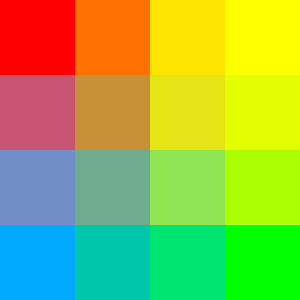
\includegraphics[width=3cm]{./fig/color.png}
            \caption{元画像}
            \label{fig:cl}
        \end{minipage}
        \begin{minipage}[t]{0.3\hsize}
            \centering
            
\includegraphics[width=3cm]{./fig/ave.png}
            \caption{$RGB$平均}
            \label{fig:cl1}
        \end{minipage}
        \begin{minipage}[t]{0.3\hsize}
            \centering
            
\includegraphics[width=3cm]{./fig/graycolor.png}
            \caption{$本研究で用いる変換$}
            \label{fig:gray}
        \end{minipage}
    \end{figure}
\section{割当問題}
    \noindent
    \textbf{3．original画像の駒とtarget画像の駒とで合成駒を生成するための組み合わせ（配置）を決める．}
    
    各駒内に含まれるピクセルの個数を$p$とし，
    original画像の$k$番目の駒の各ピクセル$i$$(1\leq i \leq p)$のグレースケール値を$org^{k}_{i}$とし，
    同様に，target画像の$l$番目の駒の各ピクセル$i$のグレースケール値を$tag^{l}_{i}$とする．
    また，original画像の$k$番目の駒とtarget画像の$l$番目の駒の距離の2乗を$dist_{kl}=\sum ^{p}_{i=1}(org^{k}_{i}-tag^{l}_{i})^2$，
    original画像の$k$番目の駒をtarget画像の$l$番目の駒に割り当てた時を$x_{kl}=1$，それ以外の時を$x_{kl}=0$と定義する．

    本研究では，$\sum ^{n^2}_{k=1}\sum ^{n^2}_{l=1} dist_{kl}x_{kl}$を最小化する最適解を求める．以下に定式化したものを示す．
    \begin{eqnarray*}
        minimize.　\sum ^{n^2}_{k=1}\sum ^{n^2}_{l=1} && dist_{kl}x_{kl} \\
        s.t.　\sum ^{n^2}_{k=1} x_{kl} &=&1 \hspace{15pt}(l=1,...,n^2) \\
             \sum ^{n^2}_{l=1} x_{kl} &=&1 \hspace{15pt}(k=1,...,n^2) \\
             x_{kl}&\in& \{0,1\} \hspace{15pt}(k=1,...,n^2，l=1,...,n^2)
    \end{eqnarray*}
    以上のような，二部グラフの両端の頂点数が等しく，完全二部グラフである場合のマッチングを求める問題は割当問題と呼ばれる．
    本研究では，この割当問題を「ハンガリー法」と呼ばれる$O(V^3)$のアルゴリズムで解く（$V$は頂点数）．
    以下で，ハンガリー法のアルゴリズムを説明する．
    
    \noindent
    \textbf{ハンガリー法}

    \begin{description}
        \item[ステップ1]\mbox{}\\ 
        各行の各要素からその行の最小値を引き，同様に各列の各要素からその列の最小値を引く．
        \item[ステップ2]\mbox{}\\ 
        各行各列から0を1つずつ選ぶことができれば，その0位置の組が割当案となる．それができなければステップ3に進む．
        \item[ステップ3]\mbox{}\\ 
        全ての0をできるだけ少ない数の縦または横の線で覆う．
        \item[ステップ4]\mbox{}\\ 
        線で覆われていない要素から，それらの最小値$min$を引き，縦横の線の重なっている要素に加え，ステップ2に戻る． 
    \end{description}
    図\ref{fig:hung}は，$k$行目$l$列目の要素を$dist_{kl}$とする行列$A$でのハンガリー法の動作例である．
    \begin{figure}[H]
        \centering
        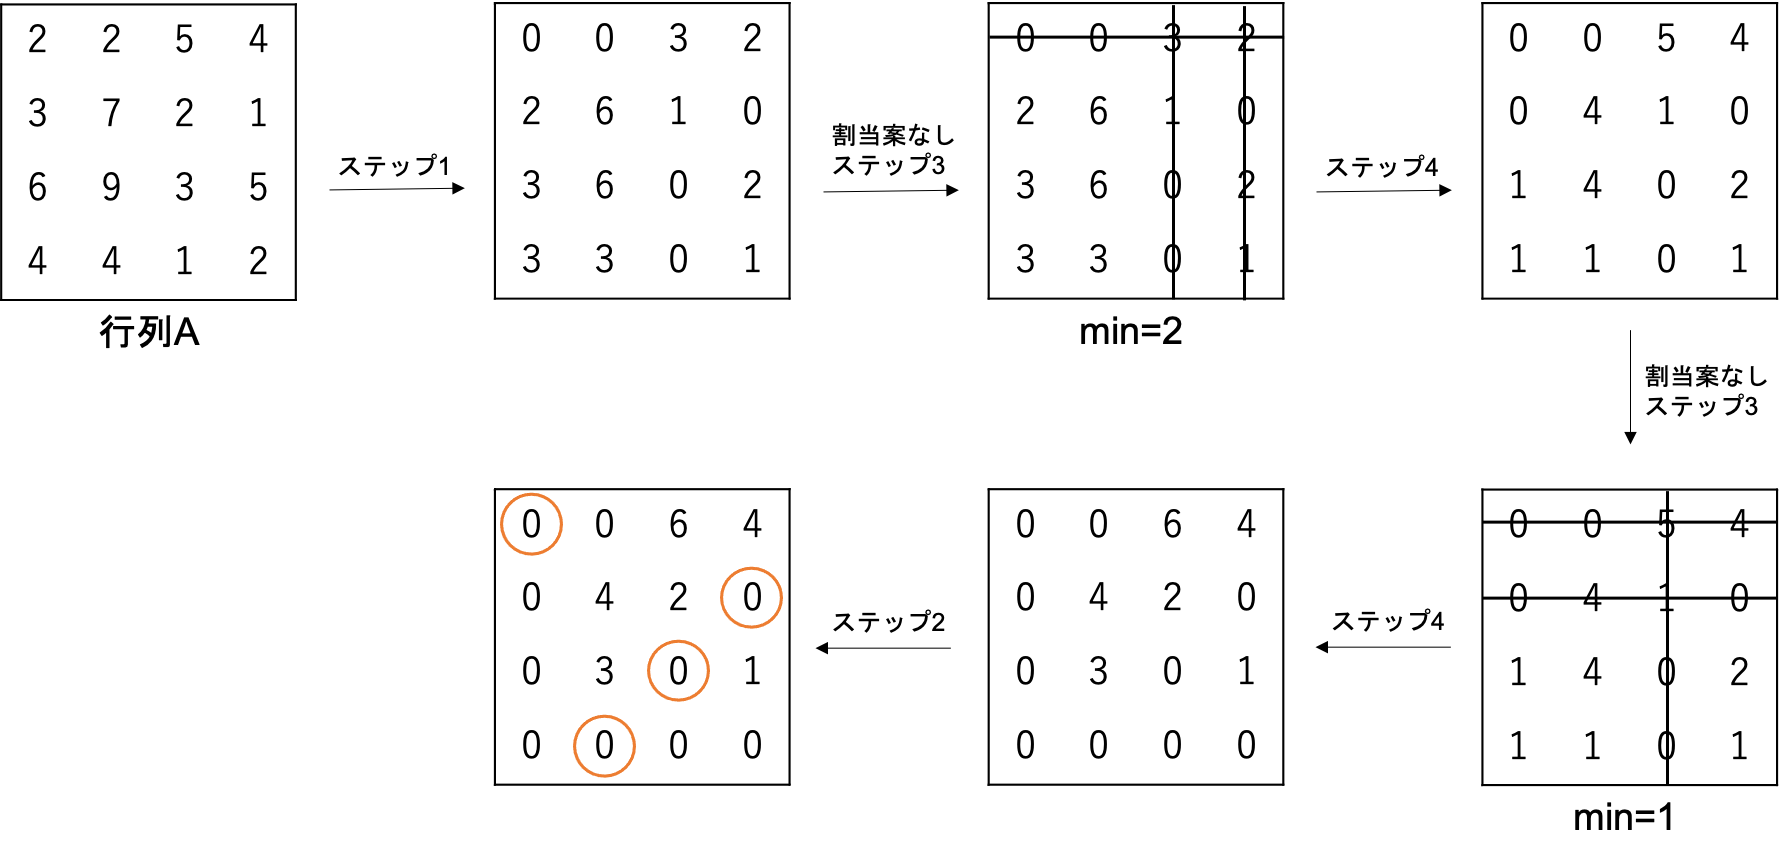
\includegraphics[width=10cm]{./fig/hung.png}
        \caption{$ハンガリー法の動作例$}
        \label{fig:hung}
    \end{figure}
    よってこの場合の最適値は，$dist_{11}+dist_{24}+dist_{33}+dist_{42}=10$となる．
\section{パズルの表示}
    \noindent
    \textbf{4．組み合わせから，$n \times n$個の合成駒を生成し，original画像に割り当てる．}
    
    $k$番目の合成駒の各ピクセル$i$のグレースケール値を$marge^{k}_{i}$，original画像の$k$番目の駒に割り当てたtarget画像の駒の番目を$alloc(k)$と定義する．
    本研究で用いる合成駒は，以下の式によって生成される．

    \begin{alignat*}{2}
        marge^{k}_{i}=\frac{(org^{k}_{i}+tag^{alloc(k)}_{i})}{2} & \quad & (1\leq k \leq n^2，1\leq i \leq p)
    \end{alignat*}
    \noindent
    \textbf{5．配置からのスライディングブロックパズルを解くアニメーションを出力する．}

    決定された配置を元に，\ref{sec:alg}項で説明したアルゴリズムを用いて，Processingのプログラムを動かす．


